\documentclass[12pt,a4paper]{article}
\usepackage{ctex}
\usepackage{amsmath, amssymb, amsthm}
\usepackage{graphicx}
\usepackage{tikz}
\usepackage{pgfplots}
\usepackage{booktabs}
\usepackage{geometry}
\usepackage{physics}
\usepackage{float}
\geometry{a4paper, left=2cm, right=2cm, top=2cm, bottom=2.5cm}

% 设置中文字体
\setCJKmainfont{AR PL UMing CN}
\setCJKsansfont{Noto Sans CJK SC}
\setCJKmonofont{AR PL KaitiM GB}

\title{\textbf{机器人学第六章:轨迹规划详细推导}}
\author{wwl}
\date{}

\begin{document}

\maketitle

\section{轨迹规划的基本概念}

\subsection{问题定义}

在机器人控制中,轨迹规划的目标是生成一个时间函数,描述机器人从初始状态到目标状态的运动过程。对于单个关节,我们考虑:

\begin{itemize}
    \item 位置轨迹:$q(t)$
    \item 速度轨迹:$\dot{q}(t) = \dfrac{dq}{dt}$
    \item 加速度轨迹:$\ddot{q}(t) = \dfrac{d^2q}{dt^2}$
\end{itemize}

给定约束条件:
\begin{align*}
    q(0) &= q_i \quad \text{(初始位置)} \\
    q(t_f) &= q_f \quad \text{(最终位置)} \\
    \dot{q}(0) &= 0 \quad \text{(初始速度为零)} \\
    \dot{q}(t_f) &= 0 \quad \text{(最终速度为零)}
\end{align*}

\section{两点间轨迹插值的详细推导}

\subsection{梯形速度曲线方法}

\subsubsection{阶段划分}

我们将运动分为三个阶段:

\begin{enumerate}
    \item \textbf{加速阶段}:$0 \leq t \leq t_c$,恒定加速度 $a_c$
    \item \textbf{匀速阶段}:$t_c < t \leq t_f - t_c$,恒定速度 $v_c$
    \item \textbf{减速阶段}:$t_f - t_c < t \leq t_f$,恒定减速度 $-a_c$
\end{enumerate}

\begin{figure}[H]
\centering
\begin{tikzpicture}
    % 速度图
    \begin{scope}[xshift=0cm, scale=1.2]
        \draw[->] (0,0) -- (5,0) node[right] {$t$};
        \draw[->] (0,0) -- (0,3) node[above] {$\dot{q}(t)$};
        
        % 梯形速度曲线
        \draw[thick, blue] (0,0) -- (1.5,2) -- (3.5,2) -- (5,0);
        \draw[dashed] (1.5,0) node[below] {$t_c$} -- (1.5,2);
        \draw[dashed] (3.5,0) node[below] {$t_f-t_c$} -- (3.5,2);
        \draw[dashed] (0,2) node[left] {$v_c$} -- (1.5,2);
        
        \node at (0.75,1) {加速};
        \node at (2.5,2.3) {匀速};
        \node at (4.25,1) {减速};
    \end{scope}
    
    % 位置图
    \begin{scope}[xshift=7cm, scale=1.2]
        \draw[->] (0,0) -- (5,0) node[right] {$t$};
        \draw[->] (0,0) -- (0,3) node[above] {$q(t)$};
        
        % 位置曲线:三段抛物线
        \draw[thick, red] (0,0.5) parabola bend (1.5,2) (1.5,2);
        \draw[thick, red] (1.5,2) -- (3.5,3);
        \draw[thick, red] (3.5,3) parabola bend (5,3.5) (5,3.5);
        
        \draw[dashed] (1.5,0) node[below] {$t_c$} -- (1.5,2);
        \draw[dashed] (3.5,0) node[below] {$t_f-t_c$} -- (3.5,3);
        \draw[dashed] (2.5,0) node[below] {$t_m$} -- (2.5,2.5);
        
        \node at (0.5,1) {抛物线};
        \node at (2.5,2.5) {直线};
        \node at (4.5,2.5) {抛物线};
    \end{scope}
\end{tikzpicture}
\caption{梯形速度曲线及其对应的位置轨迹}
\label{fig:trapezoidal}
\end{figure}

\subsubsection{步骤1:确定关键参数}

定义中点时间和位置:
\begin{align}
    t_m &= \frac{t_f}{2} \\
    q_m &= \frac{q_i + q_f}{2}
\end{align}

在加速阶段结束时:
\begin{align}
    v_c &= a_c t_c \label{eq:vc} \\
    q_c &= q_i + \frac{1}{2} a_c t_c^2 \label{eq:qc}
\end{align}

\subsubsection{步骤2:建立位移方程}

总位移等于速度曲线下的面积:
\begin{align*}
    q_f - q_i &= \text{梯形面积} \\
    &= \frac{1}{2}[(t_f - (t_f - 2t_c)) + t_f] \cdot v_c \\
    &= (t_f - t_c) \cdot v_c
\end{align*}

代入公式(\ref{eq:vc}):
\begin{equation}
    q_f - q_i = (t_f - t_c) a_c t_c \label{eq:displacement}
\end{equation}

\subsubsection{步骤3:求解加速时间 $t_c$}

将方程(\ref{eq:displacement})展开:
\begin{align*}
    q_f - q_i &= a_c t_f t_c - a_c t_c^2 \\
    a_c t_c^2 - a_c t_f t_c + (q_f - q_i) &= 0
\end{align*}

这是一个关于 $t_c$ 的二次方程,解为:
\begin{align*}
    t_c &= \frac{a_c t_f \pm \sqrt{(a_c t_f)^2 - 4a_c(q_f - q_i)}}{2a_c} \\
    &= \frac{t_f}{2} \pm \frac{1}{2} \sqrt{t_f^2 - \frac{4(q_f - q_i)}{a_c}}
\end{align*}

由于 $t_c < \frac{t_f}{2}$,我们取负号:
\begin{equation}
\boxed{
t_c = \frac{t_f}{2} - \frac{1}{2} \sqrt{t_f^2 - \frac{4(q_f - q_i)}{a_c}}
}
\label{eq:tc_final}
\end{equation}

\subsubsection{步骤4:推导各阶段轨迹方程}

\textbf{阶段1:加速阶段 ($0 \leq t \leq t_c$)}
\begin{align*}
    \ddot{q}_1(t) &= a_c \\
    \dot{q}_1(t) &= \int a_c dt = a_c t + C_1
\end{align*}
由初始条件 $\dot{q}_1(0) = 0$ 得 $C_1 = 0$,所以:
\begin{align*}
    \dot{q}_1(t) &= a_c t \\
    q_1(t) &= \int a_c t dt = \frac{1}{2} a_c t^2 + C_2
\end{align*}
由 $q_1(0) = q_i$ 得 $C_2 = q_i$,所以:
\begin{equation}
\boxed{
q_1(t) = q_i + \frac{1}{2} a_c t^2
}
\label{eq:phase1}
\end{equation}

\textbf{阶段2:匀速阶段 ($t_c < t \leq t_f - t_c$)}
\begin{align*}
    \dot{q}_2(t) &= v_c = a_c t_c \\
    q_2(t) &= \int v_c dt = v_c t + C_3
\end{align*}
在 $t = t_c$ 时,位置应连续:$q_2(t_c) = q_1(t_c) = q_i + \frac{1}{2} a_c t_c^2$
\begin{align*}
    v_c t_c + C_3 &= q_i + \frac{1}{2} a_c t_c^2 \\
    a_c t_c^2 + C_3 &= q_i + \frac{1}{2} a_c t_c^2 \\
    C_3 &= q_i - \frac{1}{2} a_c t_c^2
\end{align*}
所以:
\begin{align*}
    q_2(t) &= v_c t + q_i - \frac{1}{2} a_c t_c^2 \\
    &= a_c t_c t + q_i - \frac{1}{2} a_c t_c^2 \\
    &= q_i + a_c t_c (t - \frac{t_c}{2})
\end{align*}
\begin{equation}
\boxed{
q_2(t) = q_i + a_c t_c (t - \frac{t_c}{2})
}
\label{eq:phase2}
\end{equation}

\textbf{阶段3:减速阶段 ($t_f - t_c < t \leq t_f$)}
设 $\tau = t_f - t$,则当 $t = t_f - t_c$ 时,$\tau = t_c$;当 $t = t_f$ 时,$\tau = 0$。

减速阶段是加速阶段的逆过程:
\begin{align*}
    \ddot{q}_3(t) &= -a_c \\
    \dot{q}_3(t) &= -a_c \tau + C_4 = -a_c (t_f - t) + C_4
\end{align*}
由 $\dot{q}_3(t_f) = 0$ 得:
\begin{align*}
    -a_c (t_f - t_f) + C_4 &= 0 \Rightarrow C_4 = 0
\end{align*}
所以:
\begin{align*}
    \dot{q}_3(t) &= -a_c (t_f - t) \\
    q_3(t) &= \int -a_c (t_f - t) dt = a_c \int (t - t_f) dt \\
    &= \frac{1}{2} a_c (t - t_f)^2 + C_5
\end{align*}
由 $q_3(t_f) = q_f$ 得:
\begin{align*}
    \frac{1}{2} a_c (t_f - t_f)^2 + C_5 &= q_f \Rightarrow C_5 = q_f
\end{align*}
所以:
\begin{equation}
\boxed{
q_3(t) = q_f - \frac{1}{2} a_c (t_f - t)^2
}
\label{eq:phase3}
\end{equation}

\subsubsection{步骤5:连续性验证}

在 $t = t_c$ 处验证连续性:

位置连续:
\begin{align*}
    q_1(t_c) &= q_i + \frac{1}{2} a_c t_c^2 \\
    q_2(t_c) &= q_i + a_c t_c (t_c - \frac{t_c}{2}) = q_i + \frac{1}{2} a_c t_c^2 \quad \checkmark
\end{align*}

速度连续:
\begin{align*}
    \dot{q}_1(t_c) &= a_c t_c \\
    \dot{q}_2(t_c) &= a_c t_c \quad \checkmark
\end{align*}

在 $t = t_f - t_c$ 处验证连续性:

位置连续:
\begin{align*}
    q_2(t_f - t_c) &= q_i + a_c t_c (t_f - t_c - \frac{t_c}{2}) = q_i + a_c t_c (t_f - \frac{3}{2}t_c) \\
    q_3(t_f - t_c) &= q_f - \frac{1}{2} a_c (t_f - (t_f - t_c))^2 = q_f - \frac{1}{2} a_c t_c^2
\end{align*}

由方程(\ref{eq:displacement}):$q_f - q_i = a_c t_c (t_f - t_c)$,代入得:
\begin{align*}
    q_3(t_f - t_c) &= [q_i + a_c t_c (t_f - t_c)] - \frac{1}{2} a_c t_c^2 \\
    &= q_i + a_c t_c (t_f - t_c) - \frac{1}{2} a_c t_c^2 \\
    &= q_i + a_c t_c (t_f - \frac{3}{2}t_c) \quad \checkmark
\end{align*}

速度连续:
\begin{align*}
    \dot{q}_2(t_f - t_c) &= a_c t_c \\
    \dot{q}_3(t_f - t_c) &= -a_c (t_f - (t_f - t_c)) = -a_c t_c \quad \text{?}
\end{align*}

这里出现速度不连续!我们需要修正。

\subsubsection{步骤6:修正减速阶段的速度方程}

实际上,减速阶段应该从当前速度 $v_c$ 开始减速。正确的推导:

设 $\tau = t - (t_f - t_c)$,则:
\begin{align*}
    \ddot{q}_3(t) &= -a_c \\
    \dot{q}_3(t) &= -a_c \tau + C_6
\end{align*}
当 $\tau = 0$ 时(即 $t = t_f - t_c$),$\dot{q}_3 = v_c = a_c t_c$:
\begin{align*}
    -a_c \cdot 0 + C_6 &= a_c t_c \Rightarrow C_6 = a_c t_c
\end{align*}
所以:
\begin{align*}
    \dot{q}_3(t) &= -a_c \tau + a_c t_c = a_c (t_c - \tau) = a_c [t_c - (t - (t_f - t_c))] \\
    &= a_c (t_f - t)
\end{align*}
\begin{equation}
\boxed{
\dot{q}_3(t) = a_c (t_f - t)
}
\label{eq:velocity_phase3_corrected}
\end{equation}

现在验证速度连续性:
\begin{align*}
    \dot{q}_2(t_f - t_c) &= a_c t_c \\
    \dot{q}_3(t_f - t_c) &= a_c (t_f - (t_f - t_c)) = a_c t_c \quad \checkmark
\end{align*}

位置轨迹:
\begin{align*}
    q_3(t) &= \int \dot{q}_3(t) dt = \int a_c (t_f - t) dt \\
    &= a_c (t_f t - \frac{1}{2}t^2) + C_7
\end{align*}
由 $q_3(t_f) = q_f$:
\begin{align*}
    a_c (t_f^2 - \frac{1}{2}t_f^2) + C_7 &= q_f \\
    \frac{1}{2} a_c t_f^2 + C_7 &= q_f \Rightarrow C_7 = q_f - \frac{1}{2} a_c t_f^2
\end{align*}
所以:
\begin{align*}
    q_3(t) &= a_c (t_f t - \frac{1}{2}t^2) + q_f - \frac{1}{2} a_c t_f^2 \\
    &= q_f - \frac{1}{2} a_c (t_f^2 - 2t_f t + t^2) \\
    &= q_f - \frac{1}{2} a_c (t_f - t)^2
\end{align*}
这与之前的公式(\ref{eq:phase3})一致。

\section{多路径点轨迹规划}

\subsection{问题定义}

给定 $n$ 个路径点:$\{q_1, q_2, \dots, q_n\}$,对应时间:$\{t_1, t_2, \dots, t_n\}$。

目标:构造平滑轨迹 $q(t)$,使其经过所有路径点,且速度连续。

\subsection{线性段与抛物线过渡方法}

\begin{figure}[H]
\centering
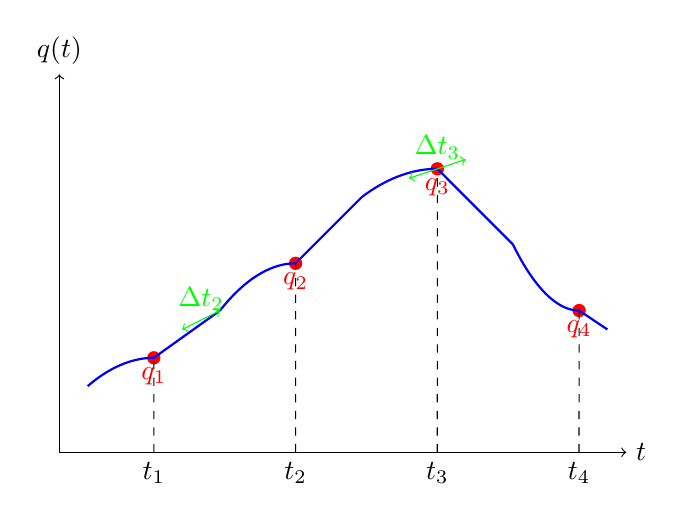
\begin{tikzpicture}[scale=1.2]
    \draw[->] (0,0) -- (6,0) node[right] {$t$};
    \draw[->] (0,0) -- (0,4) node[above] {$q(t)$};
    
    % 路径点
    \coordinate (A) at (1,1);
    \coordinate (B) at (2.5,2);
    \coordinate (C) at (4,3);
    \coordinate (D) at (5.5,1.5);
    
    \fill[red] (A) circle (2pt) node[below] {$q_1$};
    \fill[red] (B) circle (2pt) node[below] {$q_2$};
    \fill[red] (C) circle (2pt) node[below] {$q_3$};
    \fill[red] (D) circle (2pt) node[below] {$q_4$};
    
    % 时间标注
    \draw[dashed] (1,0) node[below] {$t_1$} -- (A);
    \draw[dashed] (2.5,0) node[below] {$t_2$} -- (B);
    \draw[dashed] (4,0) node[below] {$t_3$} -- (C);
    \draw[dashed] (5.5,0) node[below] {$t_4$} -- (D);
    
    % 轨迹
    \draw[thick, blue] (0.3,0.7) parabola bend (A) (A);
    \draw[thick, blue] (A) -- (1.7,1.5);
    \draw[thick, blue] (1.7,1.5) parabola bend (B) (B);
    \draw[thick, blue] (B) -- (3.2,2.7);
    \draw[thick, blue] (3.2,2.7) parabola bend (C) (C);
    \draw[thick, blue] (C) -- (4.8,2.2);
    \draw[thick, blue] (4.8,2.2) parabola bend (D) (D);
    \draw[thick, blue] (D) -- (5.8,1.3);
    
    % 过渡区域标注
    \draw[<->, green] (1.3,1.3) -- (1.7,1.5) node[midway, above] {$\Delta t_2$};
    \draw[<->, green] (3.7,2.9) -- (4.3,3.1) node[midway, above] {$\Delta t_3$};
\end{tikzpicture}
\caption{多路径点轨迹规划:线性段与抛物线过渡}
\label{fig:via_points}
\end{figure}

\subsection{数学推导}

\subsubsection{步骤1:计算直线段速度}

对于每个直线段 $[t_{k-1}, t_k]$,计算平均速度:
\begin{equation}
\dot{q}_{k-1,k} = \frac{q_k - q_{k-1}}{t_k - t_{k-1}}, \quad k = 2, 3, \dots, n
\label{eq:linear_velocity}
\end{equation}

边界条件:$\dot{q}_{0,1} = 0$, $\dot{q}_{n,n+1} = 0$。

\subsubsection{步骤2:确定抛物线参数}

在路径点 $k$ 附近,使用二次函数:
\begin{equation}
q(t) = b_{2,k} (t - t_k)^2 + b_{1,k} (t - t_k) + b_{0,k}, \quad t \in [t_k - \frac{\Delta t_k}{2}, t_k + \frac{\Delta t_k}{2}]
\label{eq:quadratic}
\end{equation}

速度函数:
\begin{equation}
\dot{q}(t) = 2b_{2,k} (t - t_k) + b_{1,k}
\label{eq:quadratic_velocity}
\end{equation}

\subsubsection{步骤3:求解系数}

在过渡区间的边界处,速度应与相邻直线段的速度匹配:

在 $t = t_k - \frac{\Delta t_k}{2}$ 处:
\begin{align}
\dot{q}(t_k - \frac{\Delta t_k}{2}) &= 2b_{2,k}(-\frac{\Delta t_k}{2}) + b_{1,k} = -b_{2,k}\Delta t_k + b_{1,k} = \dot{q}_{k-1,k}
\label{eq:boundary1}
\end{align}

在 $t = t_k + \frac{\Delta t_k}{2}$ 处:
\begin{align}
\dot{q}(t_k + \frac{\Delta t_k}{2}) &= 2b_{2,k}(\frac{\Delta t_k}{2}) + b_{1,k} = b_{2,k}\Delta t_k + b_{1,k} = \dot{q}_{k,k+1}
\label{eq:boundary2}
\end{align}

将方程(\ref{eq:boundary1})和(\ref{eq:boundary2})相加:
\begin{align*}
(-b_{2,k}\Delta t_k + b_{1,k}) + (b_{2,k}\Delta t_k + b_{1,k}) &= \dot{q}_{k-1,k} + \dot{q}_{k,k+1} \\
2b_{1,k} &= \dot{q}_{k-1,k} + \dot{q}_{k,k+1}
\end{align*}
\begin{equation}
\boxed{
b_{1,k} = \frac{\dot{q}_{k-1,k} + \dot{q}_{k,k+1}}{2}
}
\label{eq:b1}
\end{equation}

将方程(\ref{eq:boundary2})减去方程(\ref{eq:boundary1}):
\begin{align*}
(b_{2,k}\Delta t_k + b_{1,k}) - (-b_{2,k}\Delta t_k + b_{1,k}) &= \dot{q}_{k,k+1} - \dot{q}_{k-1,k} \\
2b_{2,k}\Delta t_k &= \dot{q}_{k,k+1} - \dot{q}_{k-1,k}
\end{align*}
\begin{equation}
\boxed{
b_{2,k} = \frac{\dot{q}_{k,k+1} - \dot{q}_{k-1,k}}{2\Delta t_k}
}
\label{eq:b2}
\end{equation}

加速度为:
\begin{equation}
\ddot{q}_k = 2b_{2,k} = \frac{\dot{q}_{k,k+1} - \dot{q}_{k-1,k}}{\Delta t_k}
\label{eq:acceleration}
\end{equation}

\subsubsection{步骤4:确定位置系数 $b_{0,k}$}

在 $t = t_k + \frac{\Delta t_k}{2}$ 处,位置应连续。直线段的位置为:
\begin{equation}
q_{\text{linear}}(t_k + \frac{\Delta t_k}{2}) = q_k + \dot{q}_{k,k+1} \cdot \frac{\Delta t_k}{2}
\label{eq:linear_position}
\end{equation}

抛物线段的位置为:
\begin{align}
q_{\text{quad}}(t_k + \frac{\Delta t_k}{2}) &= b_{2,k}(\frac{\Delta t_k}{2})^2 + b_{1,k}(\frac{\Delta t_k}{2}) + b_{0,k} \nonumber \\
&= \frac{b_{2,k}\Delta t_k^2}{4} + \frac{b_{1,k}\Delta t_k}{2} + b_{0,k}
\label{eq:quad_position}
\end{align}

令两者相等:
\begin{align*}
q_k + \dot{q}_{k,k+1} \cdot \frac{\Delta t_k}{2} &= \frac{b_{2,k}\Delta t_k^2}{4} + \frac{b_{1,k}\Delta t_k}{2} + b_{0,k}
\end{align*}

代入 $b_{2,k}$ 和 $b_{1,k}$:
\begin{align*}
b_{0,k} &= q_k + \dot{q}_{k,k+1} \cdot \frac{\Delta t_k}{2} - \frac{b_{2,k}\Delta t_k^2}{4} - \frac{b_{1,k}\Delta t_k}{2} \\
&= q_k + \dot{q}_{k,k+1} \cdot \frac{\Delta t_k}{2} - \frac{(\dot{q}_{k,k+1} - \dot{q}_{k-1,k})\Delta t_k}{8} - \frac{(\dot{q}_{k-1,k} + \dot{q}_{k,k+1})\Delta t_k}{4}
\end{align*}

合并同类项:
\begin{align*}
b_{0,k} &= q_k + \left[ \frac{\dot{q}_{k,k+1}}{2} - \frac{\dot{q}_{k,k+1} - \dot{q}_{k-1,k}}{8} - \frac{\dot{q}_{k-1,k} + \dot{q}_{k,k+1}}{4} \right] \Delta t_k \\
&= q_k + \left[ \frac{4\dot{q}_{k,k+1} - (\dot{q}_{k,k+1} - \dot{q}_{k-1,k}) - 2(\dot{q}_{k-1,k} + \dot{q}_{k,k+1})}{8} \right] \Delta t_k \\
&= q_k + \left[ \frac{4\dot{q}_{k,k+1} - \dot{q}_{k,k+1} + \dot{q}_{k-1,k} - 2\dot{q}_{k-1,k} - 2\dot{q}_{k,k+1}}{8} \right] \Delta t_k \\
&= q_k + \left[ \frac{\dot{q}_{k,k+1} - \dot{q}_{k-1,k}}{8} \right] \Delta t_k
\end{align*}
\begin{equation}
\boxed{
b_{0,k} = q_k + \frac{(\dot{q}_{k,k+1} - \dot{q}_{k-1,k})\Delta t_k}{8}
}
\label{eq:b0}
\end{equation}

\subsubsection{步骤5:误差分析}

在路径点 $t = t_k$ 处,实际位置为:
\begin{align*}
q(t_k) &= b_{2,k}(0)^2 + b_{1,k}(0) + b_{0,k} = b_{0,k} \\
&= q_k + \frac{(\dot{q}_{k,k+1} - \dot{q}_{k-1,k})\Delta t_k}{8}
\end{align*}

因此,轨迹误差为:
\begin{equation}
\boxed{
e_k = q(t_k) - q_k = \frac{(\dot{q}_{k,k+1} - \dot{q}_{k-1,k})\Delta t_k}{8}
}
\label{eq:error}
\end{equation}

只有当 $\dot{q}_{k,k+1} = \dot{q}_{k-1,k}$(速度连续)或 $\Delta t_k = 0$(瞬时加速)时,误差才为零。

\subsection{起点和终点的特殊处理}

为了确保轨迹精确经过起点和终点,需要对第一段和最后一段进行特殊处理。

\subsubsection{起点修正}

对于第一段,我们有:
\begin{align*}
    \dot{q}_{1,2} &= \frac{q_2 - q_1}{t_2 - t_1 - \frac{\Delta t_1}{2}} \\
    \dot{q}_{1,2} &= \ddot{q}_1 \Delta t_1
\end{align*}

其中 $\ddot{q}_1 = \text{sign}(q_2 - q_1)|\ddot{q}_1|$。

解得:
\begin{equation}
\boxed{
\Delta t_1 = (t_2 - t_1) - \sqrt{(t_2 - t_1)^2 - \frac{2(q_2 - q_1)}{\ddot{q}_1}}
}
\label{eq:delta_t1}
\end{equation}

\subsubsection{终点修正}

类似地,对于最后一段:
\begin{equation}
\boxed{
\Delta t_n = (t_n - t_{n-1}) - \sqrt{(t_n - t_{n-1})^2 - \frac{2(q_n - q_{n-1})}{\ddot{q}_n}}
}
\label{eq:delta_tn}
\end{equation}


\end{document}